\begin{multimuons-2}[enhanced, tikz={rotate=0}]{Spooky Multi-Muon Events Puzzle Physicists}
  %SubArticle}[enhanced, tikz={rotate=0}]{Spooky Multi-Muon Events Puzzle Physicists}
  \begin{multicols}{3}
    CDF recently submitted a paper that helped to explain several long
    standing puzzles associated with the production of bottom quarks
    at the Tevatron. And in addition to solving these problems,
    researchers observed something perhaps even more interesting, a
    new, bigger puzzle. 
    
    The work begins with a recent CDF measurement of the rate at which
    bottom and antibottom quarks are produced at the Tevatron. The
    analysis uses muons produced in the decay of bottom quarks to identify
    the signal events. Although previous measurements showed deviations
    from the predicted production rates, this newer, more precise
    measurement was found to agree well with the theoretical
    expectation. Interestingly, CDF found that the previous measurements
    could be explained by a source of background events that had not been
    previously identified. Earlier analyses were unable to separate this
    source of background from the bottom-quark signal, causing researchers
    to miscount the number of bottom quarks produced. 
    
    The source of these background events, whimsically called \say{ghost
    events}, is the new puzzle. The properties of this background are
    quite different than background sources that had been previously
    identified. In particular, the ghost events contain more muons than
    are expected from known background sources. 
    
    The paper is just the beginning of the story. Ghost-busters have been
    called in and are working to refine our understanding of these events
    to see whether they provide evidence for new physics beyond the
    Standard Model or whether these events exploited some lack of
    understanding of the detector. The Tevatron may still have some
    surprises in store for us, and only time will tell whether we should
    believe in ghosts.
    
%    % ========================
%    \begin{figure}
%      \begin{center}
%        \vspace{-0.2in}
%        \leavevmode
%        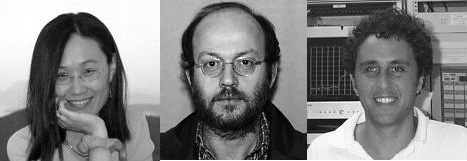
\includegraphics[width=0.5\textwidth]{./figures/Fotios-MinJeongKimBW.jpg}
%        \caption*{The following physicists played a leading role in this analysis: From
%          left to right: Min Jeong Kim, Fotis Ptohos, Fabio Happacher. Not shown: Paolo Giromini.}
%      \end{center}
%    \end{figure}
%    % ========================
  \end{multicols}
    % ========================
    \begin{figure}
      \begin{center}
        \vspace{-0.2in}
        \leavevmode
        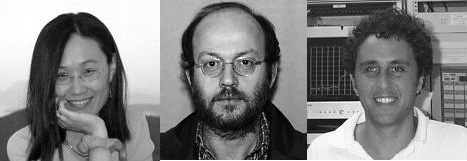
\includegraphics[width=1.0\textwidth]{./figures/Fotios-MinJeongKimBW.jpg}
        \caption*{The following physicists played a leading role in this analysis: From
          left to right: Min Jeong Kim, Fotis Ptohos, Fabio Happacher. Not shown: Paolo Giromini.}
      \end{center}
    \end{figure}
    % ========================
  
\end{multimuons-2}
